\documentclass[a4paper,11pt]{article}
\usepackage[czech]{babel}
\usepackage[a4paper, total={7in, 10in}]{geometry} % Border sizes
\usepackage[T1]{fontenc} % LaTeX default font encoding 
\usepackage{multirow} % LaTeX multirow package for table
\usepackage{titlesec} % LaTeX titlesec package for section title changes
\usepackage{sectsty} % For section styles
\usepackage{multicol} % For multi-column tables
\usepackage{graphicx} % For images
\usepackage{gensymb} % For degree /degree
\usepackage{charter} % use the charter font
\usepackage{enumitem} % Enumerated item list
\usepackage{tabularx} % For tables
\usepackage{hyperref} % For hyperlinks across the PDF
\usepackage{csquotes} % for Czech quotes
\usepackage{fancyhdr} % For headers and footers
\usepackage[bottom,norule]{footmisc} % For footnotes

% footnote in footer
\newcommand{\fancyfootnotetext}[2]{%
  \fancypagestyle{dingens}{%
    \fancyfoot[LO,RE]{\parbox{12cm}{\footnotemark[#1]\footnotesize #2}}%
  }%
  \thispagestyle{dingens}%
}

\DeclareQuoteAlias{german}{czech} % for Czech quotes
\MakeOuterQuote{"} % for Czech quotes

\sectionfont{\centering} % Center section title
\def\svgwidth{\columnwidth} % Set width of svg images to column width
\newcommand{\textoverline}[1]{$\overline{\mbox{#1}}$} % For overline on text

\sectionfont{\centering} % Center section title
\pagestyle{fancy} % Fancy page style

\begin{document}
\pagenumbering{gobble} % Remove page numbers

\section*{Maturitní otázky TVY+POS}
\begin{center}
  \Large Karel Bašta - V4D
\end{center}
\begin{enumerate}
  \item \hyperref[sec:isoosi]{ISO-OSI (význam a popis), TCP/IP (význam, popis, vztah k ISO/OSI)}
  \item \hyperref[sec:polpameti]{Polovodičové paměti (základní rozdělení, realizace buňky statické a dynamické paměti, R/W cyklus vybrané buňky)}
  \item \hyperref[sec:vlan]{VLAN (popis, struktura, činnost a návaznost na zařízení síťové vrstvy, konfigurace, subinterface, zapouzdření), význam a výhody ve vztahu k provozu na síti}
  \item \hyperref[sec:ciselnesoustavy]{Číselné soustavy, převody (celá a desetinná čísla), čísla v pohyblivé čárce (kódování)}
  \item \hyperref[sec:fyzicka-vrstva]{Fyzická vrstva (optické kabely, metalické kabely, WiFi) a zařízení}
  \item Paměti s technologií EEPROM, FLASH a SSD (princip, vícestavové ukládání, srovnání)
  \item Linková vrstva (MAC adresa a přepínaní, zařízení)
  \item Adresné módy běhu CPU (real/virtual real/protected/long, základní funkčnost, použití); výpočet adres v protected módu (fyzická/virtuální adresa, segmentování, princip výpočtu adres)
  \item Síťová vrstva (IP adresa, směrování a zařízení)
  \item \hyperref[sec:motherboard]{Motherboard (blokové schéma, účel, význam, podpůrné obvody)}
  \item Optická zařízení (druhy, princip činnosti)
  \item IPv4 adresace (classfull/classless adresace, maska, číslo sítě/ hostitele speciální adresy)
  \item Moderní CPU s integrovanými podpůrnými technologiemi (MMU- blokové schéma a využití, MMX technologie, pipelining, branch prediction)
  \item Vytváření podsítí v IPv4 (subnetting, VLSM, princip a použití)
  \item Logické členění paměti podle určení (konvenční paměť, segment, offset, page, virtuální/fyzická adresa, cache, buffer)
  \item IPv6 adresace (zápis, základní skupiny, pravidla, příklady)
  \item Činnost CPU při zpracování přerušení, DMA a podprogramu (význam, použití a rozdíly)
  \item Dynamické směrovací protokoly (rozdělení, druhy, vlastnosti a použití)
  \item Laserové a LED tiskárny (principy a technologie tisku, vlastnosti tiskáren)
  \item Rozdělení sítí podle rozsahu (PAN, LAN, WAN a topologie)
  \item Výstupní zobrazovací zařízení (CRT, plazmové, LCD a OLED monitory a projektory - princip)
  \item Hrozby na síti (viry, malware, formy a účel útoků)
  \item Aritmetické operace v počítači (operace s celými a racionálními čísly, součet/rozdíl, násobení/dělení, základní algoritmy)
  \item FW a ochrany jednotlivých vrstev TCP/IP (principy funkčnosti a nastavení, praktické příklady realizace)
  \item Vstupní zařízení (klávesnice, tablety, světelná pera, myši - princip činnosti)
\end{enumerate}

\setlist{nolistsep} % No list separator
\section{ISO-OSI, TCP/IP}
\label{sec:isoosi}
\subsection{ISO-OSI}
Problematika komunikace po síti byla tak široká, že vznikl mezinárodní refernční standard, který ji popisuje vrstvovým modelem.
Tento standard nespecifikuje realizaci, pouze její normy.
Má 7 vrstev: \\
\begin{tabularx}{\linewidth}{l|l|l|l}
  \textbf{Pořadí} & \textbf{Název} & \textbf{Data} & \textbf{Pozn.}                                                            \\
  \hline
  1.              & Aplikační      & Message       & Formátuje data pomocí protokolů (HTTP, SSH, FTP, DNS, DHCP, POP3)         \\
  \hline
  2.              & Prezentační    & Data          & Reprezentuje data a zabezpečení aplikacím (Kódování, komprese, šifrování) \\
  \hline
  3.              & Relační        & Rel. packet   & Zabezpečuje začátek a konec spojení, výměnu, integritu a korektnost dat   \\
  \hline
  4.              & Transportní    & Segment       & Zajišťuje předání paketů správné aplikaci                                 \\
  \hline
  5.              & Síťová         & Packet        & Přenos dat mezi vzdálenými počítači. Komunikace pomocí IP                 \\
  \hline
  6.              & Linková        & Frame         & Logické spojení na úrovni LAN. Komunikace pomocí MAC                      \\
  \hline
  7.              & Fyzická        & Bit           & Fyzické spojení stran (Kabely, HW, konektory \dots)                       \\
\end{tabularx}
Komunikace mezi dvěma počítači je nutné z prvního počítače vést ze sedmé vrstvy do první a následně na druhém z první vrstvy do sedmé.
\subsection{TCP}
TCP/IP je skupina protokolů pro komunikaci používané např. na internetu.
Má za úkol zajistit možnost propojení sítí založených na různých technologií.
Zajistit vysokou přenosovou rychlost na úkor spolehlivosti, jelikož o tu se starají koncové uzly již sami.
\begin{multicols}{2}
  Komunikace na TCP probíhá na: \\
  \begin{enumerate}
    \item Aplikační vrstvě
    \item Transportní vrstvě
    \item Síťové vrstvě
    \item Vrstvě síťového rozhraní
          \begin{enumerate}
            \item Fyzické vrstvě
            \item Logické vrstvě
          \end{enumerate}
  \end{enumerate}
  \columnbreak
  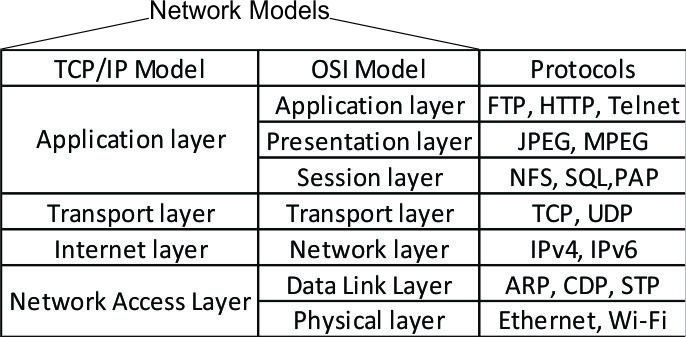
\includegraphics[height=4cm]{TVY-POS/ISO-OSI-TCP-IP/tcpip.jpg}
\end{multicols}
V koncových uzlech jsou implementovány všechny vrstvy pro kontrolu dat, v přechodových uzlech je implementována pouze síťová vrstva a vrstva síťového rozhraní.
Komunikace probíhá mezi sousedními vrstvami nebo mezi stejnolehlými vrstvami.
Pro komunikaci se používá buďto TCP, nebo UDP.
\subsection{IP}
Univerzální přenosový protokol k nespolehlivému, nespojovanému přenosu dat mezi zdrojovým počítačem a příjemcem.
Každé zařízení dostává nějakou indentifikaci v podobě IP adresy.
Přenášená data se nazývají IP datagramy neboli IP pakety, každý paket obsahuje hlavičku, ve které nese metadata a vlastní přenášená data.
Dnes se používají protokoly IPv4 a IPv6.
Cesta není předem vytyčena a optimální cestu nachází každý uzel, přes který daný paket jde.
Zpráva rozdělená na několik paketů nemusí dorazit ve stejném pořadí, jako byla poslána.
Každý poškozený paket síťová vrstva zahodí.
Požaduje-li aplikace spolehlivý přenos dat, jsou k dispozici protokoly vyšších vrstev.
Při přenosu velkých dat se mohou data fragmentovat.
Fragmentují se na vysílající stanici a defragmentují na přijímací.
\subsection{IEEE}
Jedná se o mezinárodní institum zabývající se výrobou standartů v oblasti internetového průmyslu.
Jejich protkoly se používají pro spoustu řešení v této problemice.
Od protokolu 802.1q pro trunk komunikaci ve VLAN až po 802.11 pro specikiaci WI-FI technologie.

\section{Polovodičové paměti}
\label{sec:polpameti}
Paměť je médium, které umožňuje uchovávat informace.
Základní paměťová buňka uchovává jeden bit informace - buďto logickou 0 nebo logickou 1.
Osm takových buňek tvoří jeden bajt.
Paměťové prvky jsou spojeny řádkovými a sloupcovými vodiči, pomocí kterých je možné je elektronicky ovládat.\\ \\
Parametry pamětí: \\
\begin{tabularx}{\linewidth}{l|l|l}
  \textbf{Parametr}  & \textbf{Jednotka} & \textbf{Popis}                                                        \\
  \hline
  Kapacita           & Bajt              & Množství informací, které lze do paměti uložit                        \\
  \hline
  Přístupová doba    & Sekunda           & Doba, od zadání požadavku, než paměť zpřístupní požadovanou informaci \\
  \hline
  Přenosová rychlost & Bajt za skundu    & Množství dat, které lze přečíst/zapsat za sekundu                     \\
  \hline
  Šířka toku dat     & Bit               & Počet bitů, které se po sběrnici přenášejí současně                   \\
  \hline
  Cena za bit        & Koruna za bit     & Cena za jeden bit paměti.                                             \\
  \hline
  Spolehlibost       & Sekunda           & Střední doba mezi 2 poruchami                                         \\
\end{tabularx}
\subsection{Dělení pamětí}
\subsubsection{Podle určení}
\begin{description}
  \item[Registry] - Paměti na čipu procesoru pro krátkodobé uložení dat.
    Malá kapacita, ale velmi vysoká rychlost.
  \item[Vnitřní] - Paměti na základové desce, slouží jako paměť programů a jejich data.
  \item[Vnější] - Vyměnná média a disky.
    Data jsou zaznamenávána magneticky, elektricky nebo opticky.
\end{description}
\subsubsection{Podle principu činnosti}
\begin{description}
  \item[Statická] - Pamět uchovávají informaci po dobu přívodu el. napětí.
    Mají nízkou přístupovou rychlost, ale jsou složité a drahé (Cache).
  \item[Dynamická] - Ztrácí informaci i když jsou připojené k el. napětí, proto je nutné je periodicky oživovat.
    Tvoří je transistor a kondenzátor. Mají vyšší přístupovou dobu, ale nižší náklady (Operační paměť).
\end{description}
\begin{multicols}{2}\centering
  SRAM
  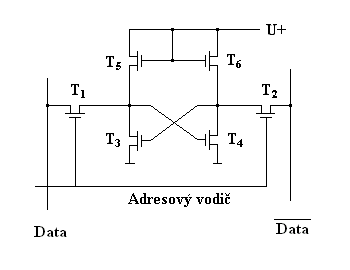
\includegraphics[width=\linewidth]{TVY-POS/Polovodicove-pameti/SRAM.png}
  \columnbreak\centering

  DRAM
  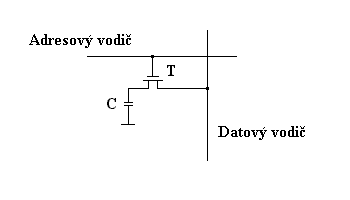
\includegraphics[width=\linewidth]{TVY-POS/Polovodicove-pameti/DRAM.png}
\end{multicols}
\subsubsection{Podle destruktivnosti při čtení}
\begin{description}
  \item[Destruktivní] - Paměť po přečtení informace ztrácí tuto informaci a je nutné ji znovu zapsat.
  \item[Nedestruktivní] - Uchovává informaci i po jejím přečtení.
\end{description}
\subsubsection{Podle energetické závilosti}
\begin{description}
  \item[Volatilní] - Paměť \textbf{NE}uchovává informaci po odpojení od el. napětí.
  \item[Non volatilní] - Paměť uchovává informaci i po odpojení od el. napětí.
\end{description}
\subsubsection{Podle přístupu}
\begin{description}
  \item[Sekvenční] - Před zpřístupněním informace je nutné přečíst všechny předcházející informace
  \item[Přímý] - Je možné přečíst přímo požadovanou informaci za pomocí její adresy
\end{description}
\subsubsection{Podle možnosti zápisu a čtení dat}
\begin{description}
  \item[ROM] - Data jsou zapsána při výrobě paměti. Realizováno vodičem nebo transistorem.
  \item[RWM] - Umožňují minimálně jeden zápis. Lze relizovat pomocí:
    \begin{itemize}
      \item PROM - Přepolování drátků. Pouze jeden zápis.
      \item EPROM - Elektronický zápis a mazání pomocí UV. Možnost více zápisů.
      \item EEPROM - Elektronický zápis i čtení. Možnost více zápisů.
    \end{itemize}
\end{description}
\subsubsection{Podle technolgie}
\begin{description}
  \item[Bipolární] - Buňky jsou tvořené bipolárními tranzistory
  \item[Unipolární] - Buňky josu tvoření tranzistory MOS
\end{description}
\subsection{R/W Cyklus buňky}
Vždy je udána adresa paměťového místa, se kterým se pracuje.
Adresa je přivedena na vstup dekoréru, která podle adresy nastaví adresový vodič na logickou 1.
Jestliže buňkou na tomto adresném vodiči projde logická 1 na datový vodič, tak je hodnota bitu logická 1.
V případě že buňkou logická 1 neprojde, pak je hodnota bitu 0.
U zápisu je dána opět adresa místa, kam se bude zapisovat, poté se nastaví hodnoty jednotlivých bitů a zapíšou se.

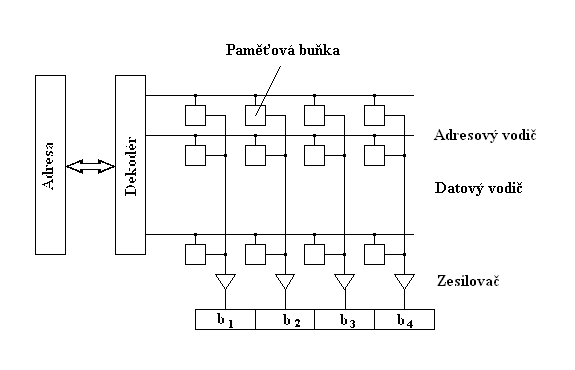
\includegraphics[width=\linewidth]{TVY-POS/Polovodicove-pameti/memorystructure.png}
\section{VLAN}
Virtuální LAN slouží k \textbf{logického rozdělení sítě nezávisle na fyzickém uspořádání}.
Lze tímto síť LAN segmentovat na menší sítě uvnitř \textbf{jedné fyzické struktury}.
Touto technologií dosáhneme výsledků, jako bychom tyto sítě měli připojené do samostného switche, ale na switchi jednom. \\
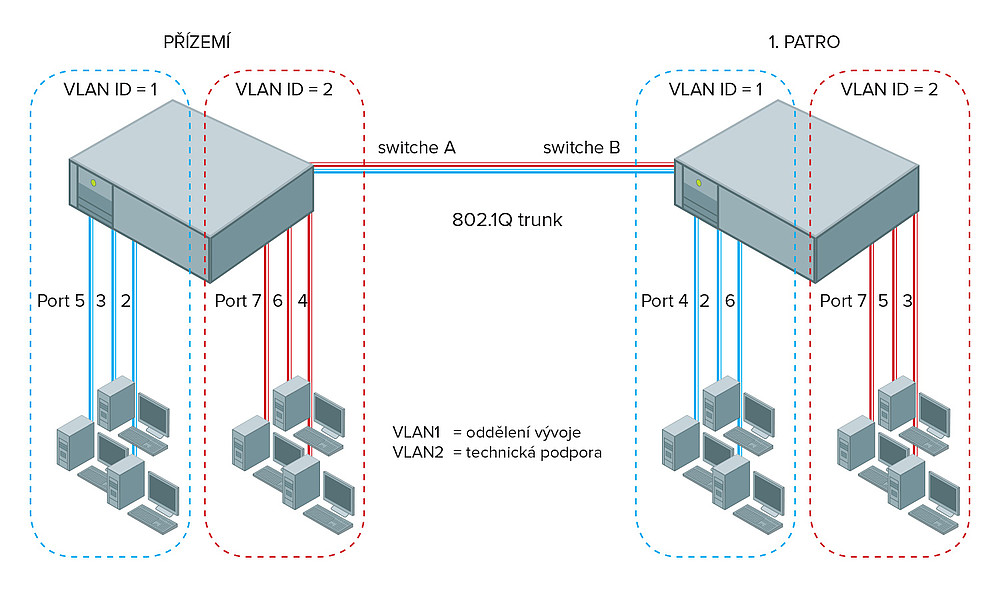
\includegraphics[width=\linewidth]{TVY-POS/VLAN/VLAN.jpg}

Tyto sítě jsou na sobě \textbf{nezávislé, nemohou spolu komunikovat}.
K zajištění komunikace mezi sítěmi \textbf{je nutno použít směrování}.
V dnešní době je možno využít \textbf{L3 switch či router}.

Jelikož komunikace po první a druhé vrstvě ISO/OSI toto rozdělení není možna zajístit, je nutné zařízením nastavit ignorování komunikace jiné sítě VLAN.
Komunikaci \textbf{je možné tímto způsobem odposlouchávat}.
Z tohoto důvodu se využívá L3 switchů a routerů schopných komunikaci \textbf{rozesílat pouze na požadované porty}. \\
\\
Důvody pro použití VLAN:
\begin{itemize}
    \item \textbf{Seskupování uživatelů} v síti podle skupin či oddělení nebo podle služeb místo podle fyzického umístění a oddělení komunikace mezi těmito skupinami
    \item \textbf{Snížení broadcast domén} v síti, které začaly být problémem již před několika lety
    \item \textbf{Zmenšení kolizních domén} v době, kdy se ještě používaly huby
\end{itemize}
Vhodné rozdělení uživatelů do VLAN:
\begin{itemize}
    \item \textbf{Podle organizační struktury} - pokud je většina komunikace v rámci oddělení, kde jsou vlastní tiskárny, file servery, \dots a mezi jednotlivými odděleními není komunikace, pouze pár služeb (mail) je společných pro všechny
    \item \textbf{Podle služeb} - do VLAN se seskupují pracovníci, kteří využívají stejné služby (Účetnictví, DB, \dots)
\end{itemize}
Výhody VLAN:
\begin{itemize}
    \item \textbf{Snížení broadcastů} - Vyšší výkon sítě
    \item \textbf{Zjednodušení správa} - K přesunu zařízení mezi VLAN je možné využít SW konfiguraci, není nutné šahat na HW
    \item \textbf{Zvýšení zabezpečení} - Oddělení komunikace, ke které poté není přístup
    \item \textbf{Oddělení speciálního provozu} - Neovlivňuje běžný provoz
    \item \textbf{Cena} (HW náročnost) - Možné využití jednoho switche pro více VLAN
\end{itemize}
\subsection{Způsoby zařezení zařízení do VLAN}
\begin{enumerate}
    \item \textbf{Podle portu} switche/routeru - Port switche má pevně stanoven jaký port přísluší jaké VLAN.
    Nejrychlejší a nejpoužívanější řešení.
    \item \textbf{Podle MAC adresy} zařízení - Switch hledá v databázi MAC adresu připojeného zařízení, podle které určuje do jaké VLAN zařízení připojí.
    Velmi náročné na výkon a administraci.
    \item \textbf{Podle protokolu} (Informací z 3. vrstvy) - Oddělení provozu podle IP adres či typu komunikace (AppleTalk)
    V praxi není příliš rozšířené.
    \item \textbf{Podle autentizace} - Zařízení se autentizuje pomocí RADIUS serveru a podle údajů se přiřadí do VLAN.
    Velmi univerzální.
\end{enumerate}
\subsection{Komunikace v rámci VLAN}
\subsubsection{Pomocí jednoho switche}
Switch si v operační paměti udržuje informace, do které VLAN patří daná komunikace a v rámci switche povoluje pouze správné směrování.
V tomto případě jsou jednotlivé porty switche buďto staticky nebo dynamicky (Podle způsobu zařazení zařízení do VLAN) zařazeny do jednotlivé VLAN.
\subsubsection{Pomocí více switchů}
Jestliže požadujeme, aby se informace o zařazení do VLAN mezi switchi neztratila, je nutné využít nějakou metodu zajišťující správný průběh.
Pokud se využívá rozdělení pomocí MAC adres zařízení, je nutné, aby si switche mezi sebou sdílely databázy MAC adres.
Firma Cisco si vytvořila vlastný metodu zvanou ISL, která přenásí informace potřebné ke správnému přenosu v rámcích komunikace, funguje ovšem pouze na zařízeních Cisco.

Nejvíce se v dnešní době používá standard IEEE 802.1Q, který značkuje rámce komunikace pouze v případě, že komunikace probíhá v rámci více switchů.
Tento standard do rámce přidává informaci o zařazení zařízení do VLAN na portu switche a na druhé straně se tato informace rozbalí a rámec se pošle správnému zařízení.
Port na kterém dochází k odchozí komunikaci do jiného switche se nazývá \textbf{trunk} port.
Spoj mezi dvěma trunk porty se nazývá \textbf{trunk} nebo \textbf{trunk link}.
\subsubsection{Native VLAN}
Na trunk portu je možné nastavit tzv. "Native VLAN", na kterém nedochází k značkování ramců komunikace.
Jestliže se na trunk port dostane rámec, který nemá tag, tak je automaticky přiřazen Native VLAN.
\subsection{Komunikace mezi VLAN}
K VLAN se můžeme chodit jako k podsítím, tudíž je možné komunikaci provádět pomocí routeru a switche, který každou podsíť připojí samostatným kabelem, nebo jedním v konfiguraci router-on-a-stick. \\
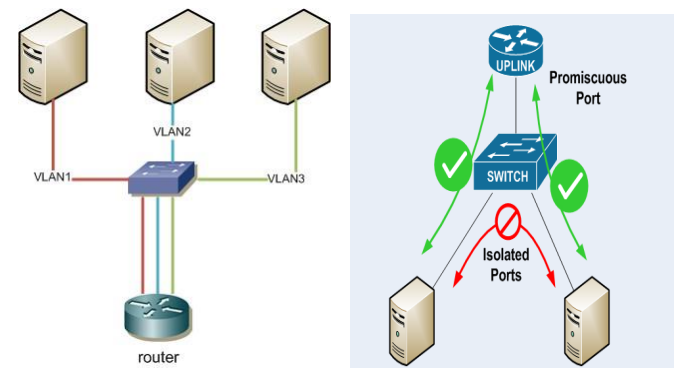
\includegraphics[width=\linewidth, height=6cm]{TVY-POS/VLAN/VLAN-router.png}
Mnohem lepší a výhodnější je ovšem využít zmiňovaných trunků a případně L3 switche, který je rychlejší.
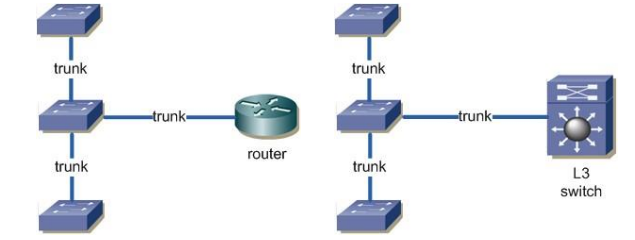
\includegraphics[width=\linewidth]{TVY-POS/VLAN/VLAN-trunk.png}
\section{Číselné soustavy, převody}
\label{sec:ciselnesoustavy}
Čísla se skládají z číslic.
Číslo 49 z číslic 4 a 9.
Reálnou hodnotu takového čísla neznáme jelikož víme že každá pozice označuje násobek základního čísla soustavy umocněné podle řádu, ale nevíme které soustavy.
V naší (desítkové) soustavě by se jednal o součet: $4*10^1 + 9*10^0$, mezitím co v jiné například: $4*16^1 + 9*16^0$.
Jestliže bychom k tomuto číslu v naší soustavě přidali 1, tak by vzniklo číslo 50, jelikož v naší soustavě nemáme čísliči větší jak 9.
Existují však soustavy, kde existují číslice větší než 9 - například F, takové soustavě se říká hexademialní a používáme ji v informatice a dokonce i soustavy kde nejvyšší číslice je 1 - takové soustavě říkáme binární a také ji používáme v informatice.
\subsection{Převody mezi soustavami}
\subsubsection{Převod z desítkové soustavy}
Z desítkové číselné soustavy převádíme do jakékoli jiné soustavy tak, že desítkové číslo dělíme základem dané číselné soustavy a sepisujeme zbytky po dělení.
Poslední získaná číslice je nejvyšší řád čísla nové soustavy.
\subsubsection{Převod desetinných míst}
Destinné číslo si rozdělíme na dvě čísla oddělené destinnou čárkou a ty samostatně převedeme a vrátíme mezi ně desetinnou čárku.
Desetinnou část ovšem místo dělení násobíme a výsledky poustupně sčítáme.
Poslední získaná číslice je nejnižší řád čísla nové soustavy.
Desetinnou část násobíme dokud nedostaneme buďto nulový výsledek, určtený počet destinných míst nebo napříkal tři nuly po sobě.
\subsubsection{Převod z binární soustavy}
Pro převod z binární soutavy do osmičkové nebo šestnáctkové soustavy rozdělujeme samotné binární číslo do trojic pro osmičkovou nebo čtveřic pro šestnáctkovou a tyto skupiny následně převádíme a řadíme za sebe podle řádu.
Pro převod do desítkové soustavy sečítáme jednotlivé hodnoty číslic.
\subsubsection{Před do binární soustavy}
Pro převod z osmičkové nebo šestnáctkové soustavy do binární musíme každou číslici převést do binární soustavy a seřadit čísla za sebou.
\subsection{Ukládání desetinných čísel}
Pro zobrazení reálných, velmi malých a nebo velmi velkých číšel se používá pohyblivá řádka.
Formát takového čísla bývá: $x = M*z^E$.
M = mantissa, E = exponent (v obrázku "fraction"), z = základ (2), x = výsledek.
K jeho zápisu nám slouží \textbf{Single precision formát}, která ukladá tyto hodnoty ve 4 bajtech paměti.\\

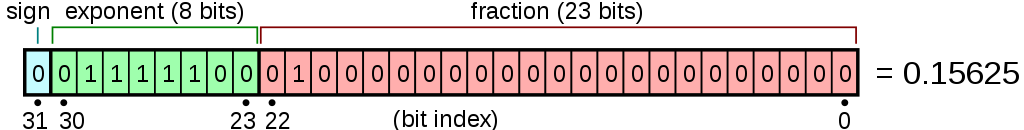
\includegraphics[width=\linewidth]{TVY-POS/Ciselne-soustavy/single_precision.png}\\

Základ čísla se neukládá, ale místo něho můžeme na posledním bitu vidět znaménkový bit pro určení záportného čísla.
Exponent se ukladá ve tvaru od -126 do 127, kde hodnota 128 představuje nulu.
Hodnoty -127 (Samé 0) a 128 (Samé 1) jsou používány pro speciální čísla (nenašel jsem).
Existují také další precision formáty, které ukládají čísla na větší místo v paměti (64bit, 128bit) určené pro přesnější čísla.

\section{Fyzická vrstva}
\label{sec:fyzicka-vrstva}
Jedná se o nijižší vrstvu ISO-OSI modelu.
Zajišťuje fyzické spojení obou stran.
Patří do ní kabeláž, HW, konektory, vysílače, příjimače aj.
Definuje elektrické, mechanické, optické a elektromagentické vlny a jejich vlastnosti.
Informace přenáší ve formě bitů - kabely, vlny a světlo neznají ale bity - je nutné definovat jaký stav znamená log. 1 a co log. 0.
Komunikace probíhá oběžníkovým způsobem a je řízena Linkovou vrstvou.
\subsection{Zařízení pracující na fyzické vrstvě}
\begin{description}
  \item[Zesilovač]- Zesiluje signál i se šumem, je jednodušší, levnější a rychlejší než opakovač
  \item[Opakovač]- Regeneruje signál (Opraví, zesílí a načasuje), elektricky odděluje segmenty
  \item[HUB (Rozbočovač)]- Navyšuje konektivitu, regeneruje signál, rozvětvuje signál do více výstupů
\end{description}
\subsection{Přenosová média}
Mezi vlastnosti přenosových médií patří:\\
\begin{tabularx}{\linewidth}{l|l|l}
  \textbf{Parametr}    & \textbf{Jednotka} & \textbf{Popis}                                      \\
  Přenosová rychlost   & Bajt za sekundu   & Množství dat, které lze přenést za sekundu          \\
  \hline
  Útlum signálu        & dB na vzdálenost  & Zeslabení signálu po průchodu určitou délkou vodiče \\
  \hline
  Odolnost vůči rušení & ---               & Zejména proti elektromagickému rušení               \\
  \hline
  Zkreslení signálu    & ---               & Jaká změna nastala na signálu po průchodu médiem    \\
  \hline
  Fyzická odolnost     & ---               & Odolnost proti ohybu, tahu, mechická pevnost        \\
\end{tabularx}
\subsubsection{Kroucená dvojlinka}
Pravidelně zkroucený pár vodičů, většinou měděných.
V dnešní době se používá několik takových navzájem zkroucených párů.
Zkroucením se minimalizuje vyzařování elektromagentických vln a minimalizují se přeslechy.
Dnes používané hojně jako Patch kabely (Ethernet).
\subsubsection{Koaxilní kabel}
Kabel s vnitřním vodičem a druhým válcovým vnějším vodičem.
Navzájem jsou vodiče odděleny dielektrikem.
Průmery kabelů jsou od milimetrů po desítky centimetrů.
Používají se pro televize.
\subsubsection{Optické kabely}
Přenášejí data pomocí světelného paprsku.
Jsou mnohem dražší a komplikovanější než metalické vodiče.
Zdrojem světla bývají LED či laserové diody.
Pro přenos ve využívá \textbf{totálního odrazu} (Fyzikální zákon, který umožňuje odrazit veškeré světlo pomocí přechodu světla z opticky hustšího prostředí do opticky řidšího)
Dělí se na:
\begin{description}
  \item[Jednovidová] - Přenáší pouze jeden světelný paprsek
  \item[Mnohovidová] - Přenáší více světelných paprsků
\end{description}
\subsubsection{Rádiové spoje}
Jedná se o přenosy elektromagentických vln v určitém rozsahu elektromagentického spektra.
Hlavní výhodou tohoto spoje je absence kabelů, tudíž bezdrátová komunikace.
Nevýhodou je možnost oblivnění přenosu pomocí vlivů, které by u drátové nebyly problém.
Pro rádiové spoje se využívá různých frekvečních délek například 87.6 Mhz (Rádio Impuls) a 5 Ghz (Wi-Fi).
Mezi další technologie hojně využívající rádiové spoje patří: Bluetooth, Mobilní signál, GPS aj.
\subsection{Druhy možností šíření signálu}
\subsubsection{Sériové a paralelní přenos}
\begin{description}
  \item[Sériové spoje]- Bity jdou za sebou postupně jedním vodičem. Bajty jsou tvořeny posloupností bitů.
  \item[Paralelní spoje]- Několik bitů se posílá současně pomocí více vodičů. Obvykle se přenáší celý bajt.
\end{description}
\subsubsection{Synchronní a asynchronní přenos}
\begin{description}
  \item[Synchronní spoje]- Přenos dat probíhá společně se signálem CLK, který generuje pouze jedna strana.
  \item[Asynchronní spoje]- Každá strana si CLK generuje sama. Komunikace začíná pomocí start a stop bitu.
\end{description}
\subsubsection{Symetričnost singálu}
\begin{description}
  \item[Symetrický signál]- Přenos probíhá dvou vodičím v opačné polaritě. Výstupní signál je rozdíl přenosů.
  \item[Asymetrický signál]- Přenos probíhá po jednom vodiči. Náchylné na poruchy, nižší spolehlivita.
\end{description}
\section{EEPROM, FLASH a SSD}
\subsection{EEPROM - Electrically Erasable Programable Read Only Memory}
Chová se podobně jako EPROM, ale data je možné smazat elektricky.
Programování je tudíž možné přímo v systému a naprogramování trvá méně než minutu.
Pro výrobu se využívají speciální tranzistory s vrstvou nitridu křemíku a oxidu křemičitého mezi kterým je uchován el. náboj, který se vkládá na jejich přechod.\\

\subsection{FLASH}
Obdoba EEPROM paměti.
Jsou to paměti statické a elektricky nezávislé.
Programují se přímo v počítači.
Paměti není nutné z počítače pro programování vyjmout.
Zapisuje so do ní po blocích a celá pamět se zapíše v rámci sekund.
Pracuje se s nimi jako s pamětmi RAM, ale po odpojení se jejich obsah nesmaže.
Při použití k uložení BIOSu, tak se BIOS dá aktualizovat.
Existují dva základní typy těchto pamětí, podle použitých logických hradel.
\subsubsection{NOR Flash paměť}

\subsubsection{NAND Flash paměť}
\subsection{SSD}
Paměti, využívané v dnešních počítačích jako nástpuce pevných disků.
Používají se zde paměti typu SRAM či DRAM.
Většinou se pro ně používají rozhraní SATA či PCIe.
Nemají žádné pohyblivé části, což znamená nižší spotřebu.
Mají rychlejší přístup k datům a mají větší přenosové rychlosti.
Podle použitých čipů mají jsou buďto dražší s vyšší životností nebo levnější s kratší životností.
Čipy:
\subsubsection{SLC}
Na každé paměťové buňce je jeden bit.
Výhodou je vyšší rychlost a menší spotřeba.
\subsubsection{MLC}

\section{Linková vrstva}
\section{Adresné módy běhu CPU}
\section{Síťová vrstva}
Zajišťuje přenos dat mezi vzdálenými počítači (WAN).
Klíčovým prvkem v této komunikaci je směrovač (router).
Každý takový směrovač má svoji jednoznačnou identifikaci v rámci WAN (IP Adresu).
Přenáší se IP datagramy neboli pakety. Nezajímá se o protokoly linkové a fyzické vrstvy.\\
Funkce síťové vrstvy:
\begin{itemize}
  \item Hledání cesty pro pakety mezi libovolnými dvěma uzly v síti
  \item Nestará o spolehlivost, ale o co nejrychlejší přenos dat
  \item Zajistění postupného přenosu paketů přes mezilehlé uzly v cestě
  \item Přenosový protokol IP se snaží zakrývat rozdíly v technologiích nižší vrstvy
\end{itemize}
Cesta paketu:
\begin{enumerate}
  \item Zabalení přenášeného paketu do rámce
  \item Prostřednictvím vrstvy síťového rozhraní předání rámce přímému sousedovi
  \item V sousedním uzlu přijmutí a rozbalení rámce vrstvou síťového rozhraní
  \item Předání získaného paketu své síťové vrstvě, která najde nejvhodnější cestu k cíli
  \item Prostřednictvím vrstvy síťového rozhraní zaslání rámce k dalšímu uzlu
\end{enumerate}
\subsection{Směrování}
Technika k vnitřnímu rozčlenění rozsáhlých sítí LAN i MAN.\\
Běžně se používá jako proces šíření globální síťové komunikace v Internetu.\\
Účely směrování:
\begin{itemize}
  \item Usměrnění komunikace
  \item Optimalizace zátěže sítě
  \item Implementace bezpečnosti
  \item Zvýšení spolehlivosti na síťové vrstvě
\end{itemize}
\begin{description}
  \item[Statické]je nastaveno pevně administrativně - DHCP
  \item[Dynamické]je pravidelně aktuailzováno speciálními protokoly - Mnoho
\end{description}
\subsection{IP Adresace}
Každá síťová stanice musí mít pevně stanovenou identifikaci - IP adresu.
Ta je buďto napevno přidělena nebo dynamicky přidělována.
V současné době se využívá IPv4 adresa o velikosti 32bitů.
Tato IP adresa má v sobě zahrnuté jak číslo sítě, tak číslo stanice.
Tvar adresy je \[XXX.XXX.XXX.XXX\]
V každé síti musí být jedinečný router, který síť propojuje pomocí směrování. IP adresa hostitele a routeru musí být odlišná.\\
Jiné protkoly dostupné pro síťovou vrstvu: ICMP - Internet Control Message Protocol (Řešení problémů IP, ping\dots), IGMP, ARP, RARP.

\section{Motherboard}
\label{sec:motherboard}
Deska plošných spojů, která elektricky a fyzicky propojuje jednotlivé komponenty počítače.
Funkce základní desky:
\begin{enumerate}
  \item Napájet komponenty
  \item Mechanicky udržet komponenty u sebe
  \item Umožnit rychlý a spolehlivý přenos dat z jedné periférie do druhé
\end{enumerate}
Možnosti zapojení komponent k základní desce:
\begin{itemize}
  \item Interně - Porty a vstupy uvnitř case na základní desce
  \item Externě - Porty a vstupny z vnější strany case, taktéž na zákldní desce
\end{itemize}
Základní desky nejsou jenom v počítačích, ale i noteboocích, mobilech aj.\\
Velikosti základních desek: E-ATX, ATX, mATX, ITX\dots
\subsection{Blokové schéma a jednotlivé komponenty}
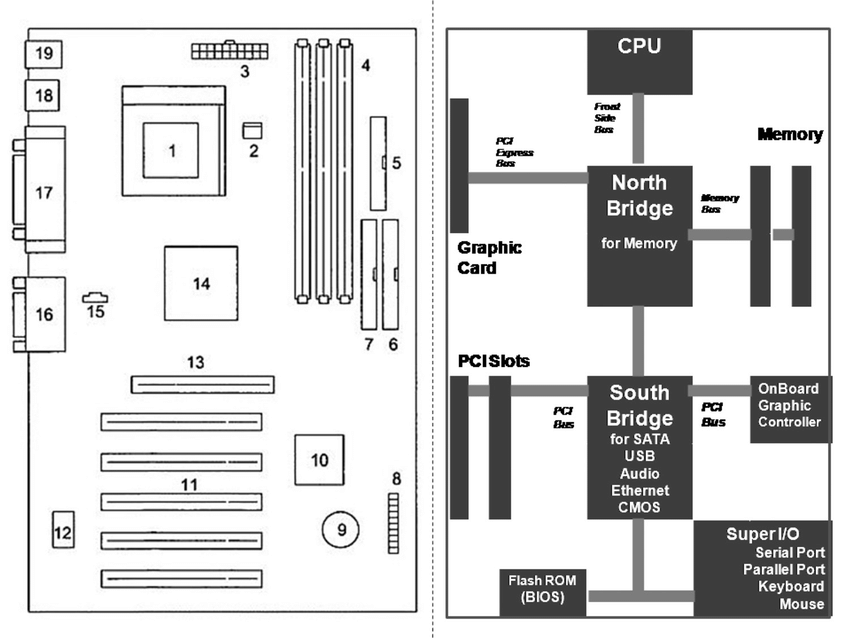
\includegraphics[width=1\linewidth,height=0.58\linewidth]{TVY-POS/Motherboard/MB.png}
Popis fyzického schéma:\\
\begin{enumerate}
  \item[1)] Patice CPU - Rozdíl mezi AMD (AM4, AM3) a Intel (12th gen LGA1700)
  \item[2)] CPU FAN Header - Pro chlazení CPU, jiné usazení chladiče pro AMD a Intel
  \item[3)] ATX napájení - Napájení základní desky a jejich komponent
  \item[4)] DDR sloty - Rozdíl mezi DDR3, DDR4, DDR5 (Umístění mezery)
  \item[8)] Porty pro case - HD Audio, USB, PWR, Reset, HDDLED, PWRLED
  \item[9)] RTC - Hodiny reálného času, baterie + kondenzátor, 32.768 kHz, 1.7 sekundy chyba denně
  \item[10)] Southbridge - Propojení NB a Serial \& Paralel port, PS2 klávesnice, myš
  \item[11)] PCI - Univerzální rozšiřující sloty. x4, x8, x16
  \item[12)] BIOS - Flash pamět se zaváděcím systémem
  \item[13)] PCI-E - Vysokorychlostní rožšiřující slot, v dnešní době hlavně pro grafické karty.
  \item[14)] Northbridge - Rozhraní pro propojení CPU s opereační pamětí a PCI-E
  \item[15)] FAN Header - Napájení a ovládání
  \item[] CPU napájení - Chybí na obrázku
\end{enumerate}

\section{Optická zařízení}
\label{sec:opticka-zarizeni}
Optické zařízení je médium uchovávající informace při jehož čtení se využívá zdroje světla.
V dnešní době se jedná o 12cm disky s dírou 1.5cm uprostřed a tlouštku 1.2mm.
Skládají se většinou ze tří částí:\\
\begin{enumerate}
  \item Směs polykarbonátu a polymethylmethakrylátu s vytlačenou spirálou pro data
  \item Reflexní vrstva pro odrážení světla laseru
  \item Ochranná vrstva - lak, potisk\dots
\end{enumerate}
\subsection{Druhy optických zařízení}
\subsubsection{CD}
Nejstarší optické médium.
Využívá vlnovou délku 870nm (Červená).
Má maximální velikost 650 MB, rychlost v násobcích 150kB/s a zapisuje se pouze na jedné straně.\\
\begin{description}
  \item[CR-ROM]- Pouze pro čtení, rychlost otáčení buďto konstatní nebo u okraje rychleji, lisování podle matice
  \item[CD-R]- Umožňuje jednorázoví zápis, poté funguje jako CD-ROM, speciální 4x rychlejší a silnější laser.
  \item[CD-RW]- Dovoluje opakovaně zapisovat data. Datová vrstva buďto krystalizuje nebo se mění na amorfní.
  Obodoba prohlubní a mezery pro zápis. Zápis zahřátím, čímž se převede disk do amorfního stavu.
\end{description}
\subsubsection{DVD}
Nástupce CD. Má větší kapacitu pomocí větší hustoty zápisu.
Využívá přesnější laser 660nm (Stále červená).
Má možnost oboustranného zápisu či dvouvrstvého provedení.
Spirála pro data je stejně dlouhá a široká jak u CD.
Pro zápis na pouze jednu z vrstev laser zaostří pouze na jednu, spodní vrstva je polo transparentní.
Má stejnou tloušťku pomocí poloviční tloušťky nosných vrstev.
Přenosová rychlost je v násobních 1350 kB/s.
Mechanika pro DVD měla dvakrát přesnější čtecí hlavy, po změně vlnové délky bylo nutné ovšem do mechanik přidávat laser pro čtení CD zvlášť.
\subsubsection{DRM}
DVD přineslo možnost DRM (Digital Rights Management) pro ochranu dat.
Na disku lze uložil copyright, který se při kopirování nepřenáší s číslem regionu.
Čtení bylo poté možné pouze jestliže na disku je nacházel tento copyright a pouze ve správném regionu.
\subsubsection{Blu-ray}
Nejmodernější optické médium.
Využívá nejmenší vlnovou délku 405nm (Modrá).
Tudíž má i vetší hustotu zápisu a větší kapacitu (Jedna datový vrstva 25GB).
Datová vrstva je blíže pod povrchem, aby nedocházelo k rozptylu laseru, ovšem to znamená menší odolnost vůči škrábancům.
Existují přepisovatelné a i menší verze disku.
Rychlosti v násobku 4.5MB/s.
\subsection{Čtení}
Mechanika obsahuje laser, která za pomocí čoček zaostřuje na disk.
Tento laser poté veden podel spirály v první vrstvě disku.
Odrázené světlo se vrací do senzoru za polopropustným zrcadlem.
Záznam proveden pomocí různě dlouhých prohlubní oddělený mezerami.
Přechod mezi prohlubní a mezerou je log. 1.
Delší prohlubeň či mezera je log. 0.

\section{IPv4 adresace}
\section{Moderní CPU s integrovanými podpůrnými technologiemi}
\label{sec:moderni-cpu}
Integrované podpůrné technologie CPU urychlují komunikaci procesoru s obovody základní desky počítače.
Mezi další výhody integrovaných podpůrných technologií je odlehčení procesoru nebo dokonce jeho zastoupení.
\subsection{MMU - Memory Management Unit}
Slouží jako vrstva mezi CPU a operační pamětí.
Hlavní funkce jsou:
\begin{itemize}
  \item Překlad virtuální adresy na fyzickou
  \item Správa virtuální paměti
  \item Rozdělení virtuálního prostoru na stránky/segmenty
\end{itemize}
Překlad adresy musí být bezpečný, rychly a umožňovat rychlé přepínání kontextu.
\subsubsection{TLB - Translation Lookaside Buffer}
Součást MMU, která ukládá v sobě nedávné překlady z virtuální paměti na fyzickou.
Když bude znova překlad potřeba, použije se rychlejši přístupný překlad v TLB.
\subsection{MMX - Multi Medial eXtension}
Aplikace využívající zvuk a video, 3D grafiku a animace.
Práce s těmito prvky se provádí ve velkých blocích dat, kde se vykonávají jednoduché repetetivní operace.
Proto se pro zrychlení práce s multimédií využívá \textbf{SIMD (Single Instruction, Multiple Data)} technologie.
Tato technologie popsiuje schopnost několika prvků provádět stejnou operaci na různých datech paralelními výpočty.
Kvůli lepší kompatibilitě jsou MMX registry aliasy pro instrukční sady x87 pro opreace s floaty.
\subsection{Cache}
Jedná se o velice rychlou SRAM paměť zabudouvanou do CPU.
Paměť cache umožňuje vyhnout se opakovanému pomalému procesu, na který bychom museli čekat.
Místo toho provedeme víc takových procesů najednou a poté tyto data nahrajeme do pamětí cache.
Mimo nahrávání dat lze do cache nahrát i instrukce pro omezení potřeby je překládat.
Jinak také cachujeme data z DRAM, které dostáváme z MMU.
\subsection{Pipelining}
Snaží se uspořádat instrukce tak aby byl procesor nejefektivněji využit.
Rozdělí příchozí instrukce na po sobě jdoucí kroky, které pak přiřadí správným částem procesoru k vykonání což umožňuje paralelní zpracování různých instrukcí.
Častou praktikou je aby se liché operace prováděli na jedné hraně hodin a sudé na druhé.
Správně nakonfigurovaný pipeline dokončí jednu instrukci každý cyklus.
Tento problém nemusíme řešit při programování ve vyšších jazycích jak assembler.
\subsection{Branch prediction}
Jakmile v rámci procesu dojde k rozhodování mezi více možnostmi, vytváří se různé větve, kterými se proces můžet vydat.
CPU neví, po které větvi se vydá, kvůli tomu musí čekat než dostane výsledek.
Pokud se snažíme předpovědět větev:
\begin{itemize}
  \item Uhodneme správně - navýšení rychlosti
  \item Uhodneme špatně - ještě větší zpomalení kvůli zbytečné práci
\end{itemize}
Rozdělení na dvě větve je většinou řešeno tak, že se druhá větev načte na jiné místo v paměti programu, a pokud je splněna podmínka pro přepnutí větvě, tak provedem skok na toto jiné místo.
Jestli ne, pokračujeme ve staré větvi.
Dynamický branch predictor si uchovává kolikrát se na daném skoku skočilo na jinou větev a kolikrát ne, podle těchto nasbíraných dat se snaží uhodnout zdali skoční neb one.
\section{Vytváření podsítí v IPv4}
\label{sec:podsite-ipv4}
Problematika sítí IPv4 je malý počet adres.
Tyto adresy je možné tedy rozdělit na podsítě, které můžeme mít přesně tak velké jak potřebujeme a nemusíme tedy zabírat zbytečně prostor, který bychom mohli využít někde jinde.
Tyto podsítě poté od sebe odlišeujeme stále logickou adresou společně s maskou sítě.
Podsítě v IPv4 se tvoří pomocí dvou způsobů:
\subsection{FLSM - Fixed Length Subnet Mask}
Rozdělení adresného prostoru mezi stejně velké podsítě každou se stejnou maskou.
Využitelné v geograficky omezené oblasti (Velké organizace, univerzity).
Síť s maskou /24, můžeme rozdělit na 2, 4, 8, 16, 32, 64 stejně velkých podsítí.
\subsection{VLSM - Variable Length Subnet Mask}
Rozdělení adresného prostoru mezi podsítě, kde má každá podsíť masku velkou jak je potřeba.
\subsection{Efektivnost technologií}
Efektivnost VLSM bývá mnohem vyšší jelikož je možné vytvořit sítě specificky velké, jak jsou potřeba.
Můžeme se setkat s případy kde by vyřešení podsítí pomocí FLSM nebylo možné i přestože by to pomocí VLSM možné bylo. \\
\subsection{Postup při tvoření podsítí}
\begin{multicols}{2}
  \begin{center}
    Máme IP adresu: \textbf{172.16.32.0/24}
  \end{center}
  \begin{enumerate}
    \item Najdeme největší podsíť. (60)
    \item Pro tuto síť určíme počet bitů potřebných pro umístění všech stanic + 2 pro router a broadcast. (6 bitů pro 62 adres)
    \item Pomocí tohoto vypočítáme masku sítě. (32 - 6 = 26 bitů)
    \item Určíme počet sítí. (4)
    \item Maska podsítě je u FLSM stejná, pro VLSM se mění pro každou podsíť v závislosti na prvních třech krocích.
  \end{enumerate}
  \columnbreak
  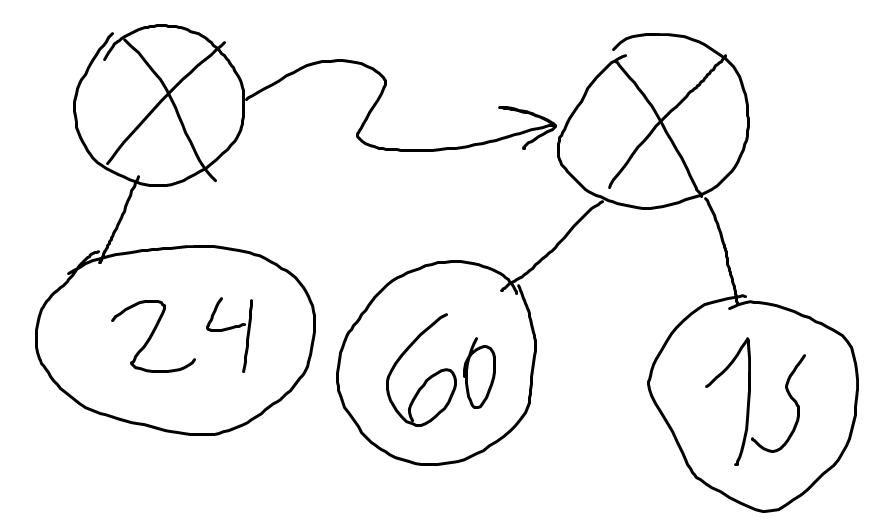
\includegraphics[width=\linewidth]{TVY-POS/Podsite-IPv4/podsit.png}
\end{multicols}
\begin{enumerate}
  \setcounter{enumi}{5}
  \item V posledním bajtu adresy IP zkontrolujeme realizovatelnost podsítí. (2 bity pro 4 masky)
  \item Poté určíme samotné masky podsítí. (00, 01, 10, 11)
  \item Určíme adresy podsítí s maskou. (127.16.32.0/26, 172.16.32.64/26, \dots)
  \item Určíme rozsah adres pro hostitele. (<1;62> 0 je adresa sítě a 63 broadcast)
  \item Podle velikosti určíme pořadí sítí.
  \item Infrastuktury (Routery a switche) sítí budou dostávat nejvyšší možnou adresy v dané podsíti.
  \item Servery dostávají zpravidla nejnižší možnou adresu v dané podsíti.
  \item Zbytek adres se rozdělí pomocí DHCP mezi běžné uživatele.
\end{enumerate}

\[\text{Efektivnost} = \frac{\text{Počet adres využitých}}{\text{Počet adres možných}}\]

\section{Logické členění paměti podle určení}
\label{sec:logicke-cleneni-pameti}
Paměť je médium, které umožňuje uchovávat informace.
Pro každé prostředí je potřeba paměť s jinou specifikací.
Jinde jsou potřeba paměti s velmi vysokou rychlost, někde s velmi krátkou přístupovou dobou nebo s velmi velkou kapacitou.
V počítači používáme následující paměti:
\subsection{Konvenční paměť}
Bývalé označení paměti v DOS, která měla 640 kB.
Sloužila pro aplikace a pracovalo se v ní v Realném režimu.
Zbytek paměti byl určet pro rozšiřující karty.
\subsection{Cache}
Jedná se o velmi rychlou paměť malé kapacity.
Slouží ke zrychlení toku dat mezi CPU a RAM.
Na procesoru se jich nachází více a každá z nich má svůj řadič.
Od Bufferu se liší tím, že může uložená data poskytovat opakovaně.
V procesoru se mohou nacházet až tři vrstvy L + číslo cache pamětí (L1, L2, L3).
Tyto paměti slouží k ukládání právě zpracovávaných instrukcí a dat.
Stupňují se s rychlostí a kapacitou.
L1 je nejrychlejší ale nejmenší.
L3 je naopak nepomalý, ale největší. 
I přesto ale je její rychlost neporovnatelná s rychlostí konvenční paměti.
\subsubsection{Asociativnost cache}
\begin{description}
  \item[Asociativní]- Vyhládáví v paměti pomocí klíče
  \item[Nesociativní]-  Vyhledávání v paměti pomocí adresy
\end{description}
\subsubsection{Adresace cache}
\begin{description}
  \item[Virtuální]- Vyhledávání podle logické adresy
  \item[Fyzická]- Výpočet fyzické adresy a až poté vyhledávání v paměti
\end{description}
\subsubsection{Synchronnost cache}
\begin{description}
  \item[Synchronní]- CPU po zadání adresy nečeká na data. Požádá o ně v dalším taktu. Odpadá čekání.
  \item[Asynchronní]-  Sběrnice je obsazena celou dobu přenosu. Nepouživá se.
\end{description}
\subsection{Buffer}
Buffer neboli vyrovnávací paměť má za úkol vyrovnat rychlosti, jesltiže vstupní data přicházejí moc rychle nebo sporadicky.
Pro práci s daty potřebujeme konstatní datovou rychlost a tu nám v takovém případě poskytuje Buffer.
Paměť je typu FIFO, tudíž první data, která do paměti přijdou, z ní také první odejdou.
Tyto data už poté nelze z této paměti získat znova.
\subsection{Segment}
Segment je část operační paměti, která je určena pro jeden konkrétní účel.
Délka tohoto segmentu je určena podle takového účelu.
Při výpočtu adresy paměti je k této informaci ještě potřeba zjisit offset, aby bylo možné z takového segmentu vybrat pouze potřebnou část dat.
\subsection{Page}
Stránkování paměti je proces, který rozdělí operační pamět na stejně dlouhé úseky o malé velikosti.
Tyto úseky poté přiděluje jednotlivým procesům v množství, ve kterém potřebují.
Tyto úseky je možné narozdíl od segmentu rozdělit po celé operační paměti a není nutné, aby byl přidělován celý blok v jednotném tvaru.
Pro aplikace se jeví paměť poté jakože má k dispozici paměť od 0 až po maximum -1.
Adresa se musí překládat pomocí MMU.
Velmi efektivní způsob rozdělení paměti.


\section{IPv6 adresace}
\section{Činnost CPU při zpracování přerušení, DMA a podprogramu}
\section{Dynamické směrovací protokoly}
\subsection{Úvod}
Pro přesun paketů ze zdroje na požadované zařízení na lokálních sítích se dnes využívá routererů, které si vytváří tzv. směrovací tabulku, pomocí které vybírají nejlepší cestu pro tento paket.
V této tabulce je možné najít:
\begin{itemize}
    \item Adresu sítě (Na které je požadované zařízení)
    \item Typ cesty (Přímá, statická či dle prokolu)
    \item Fyzické rozhraní, po kterém se paket přenese
\end{itemize}
Mezi typy cest patří:
\begin{enumerate}
    \item Přímo připojené (C)
          \begin{itemize}
              \item Není nutno konfiguovat
              \item Přidají se automaticky je-li rozhraní aktivní
              \item Administrativní vzdálenost: 0
          \end{itemize}
    \item Statické (S)
          \begin{itemize}
              \item Zadávána ručne
              \item Je nutno specifikovat IP adresu sítě s maskou a rozhraní routeru
              \item Případně lze specifikovat IP adresu protějšího routeru a směr
              \item Administrativní vzdálenost: 1
              \item Využívají se pro:
                    \begin{itemize}
                        \item Připojení sítě do Internetu pomocí jednoho ISP
                        \item Větší sítě v konfigurace „Hub-and-spoke“
                    \end{itemize}
          \end{itemize}
    \item Dynamické (Dle protokolu)
          \begin{itemize}
              \item Generují se automaticky a dynamicky
              \item Routery si navzájem sdílí informace o těchto tabulkách, podle kterých upravují vlastní
          \end{itemize}
\end{enumerate}
\subsection{Rozdělení protkolů}
Protkoly se v základu dělí na:
\begin{itemize}
    \item IGP - Používané v rámci jedné domény
    \item EGP - Používané v rámci ISP na WAN
\end{itemize}
Dělí se také ale podle dělí podle využití masky sítí na:
\begin{itemize}
    \item Classfull - Nevyuživá masky sítí, nemohou být použity ve VLSM
    \item Classless - Využívá a vyžaduje masky sítí
\end{itemize}
Samotné IGP protokoly se poté dělí na:
\begin{itemize}
    \item Protkoly měřící vzdálenost a směr (DVRP - Distance Vektor Routing Protocol)
    \item Protkoly měřící stav linek a topologickou mapu sítě (LSRP - Link State Routing Protocol)
\end{itemize}
\subsection{Distance vector protokoly (DVRP)}
Cesta je určena vektorem, ve kterém hrají role vzdálenost a směr.
Vzdálenost je určena \textbf{počtem hopů}.
Směr je určen výstupním rozhraním routeru nebo naopak adresou vstupu vedlejšího routeru.
K určení cesty se používá \textbf{Bellman-Ford} algoritmu.
Tento algoritmus neumožňuje routerům znát skutečnou mapu síťové topologie.
Některé protokoly pravidelně rozesílají kompletní směrovací tabulky všem sousedům, čímž způsobují velkou zátěž na lince.
\subsection{Link state prokoly (LSRP)}
Cesta je určena stavem linek.
Každý router zná tímto způsobem celou topologii sítě a pomocí toho generují nejlepší cestu.
Síť se zde zatěžuje velmi méně, jelikož místo rozesílání celých tabulek se zde rozesílají pouze aktualizace stavu jednotlivých linek.
Vhodné pro větší a rozsáhlejší sítě.
\subsection{Konvergence}
Jedná se o dobu, za kterou se na všech routerech vytvoří platné a nejlepší směrovací tabulky.
Mezi parametry důležité pro konvergenci patří rychlost šíření informací a rychlost výpočtu optimálních cest.
\subsection{Metrika protkolů}
\begin{tabularx}{\linewidth}{l|l}
    \textbf{Parametr} & \textbf{Popis}                     \\
    \hline
    Počet hopů        & Počet routerů mezi zdrojem a cílem \\
    \hline
    Šířka pásma       & Propustnost linky                  \\
    \hline
    Zátěž             & Zatížení linky                     \\
    \hline
    Zpoždění          & Doba průchodu paketu linkou        \\
    \hline
    Spolehlivost      & Pravděpodobnost chyby linky        \\
    \hline
    Cena              & Určeno politikou linky             \\
\end{tabularx}
\subsection{Tabulka protokolů}
\begin{tabularx}{\linewidth}{l|l|l|l|l}
    \textbf{Název (IPv6 verze)}           & \textbf{Zkratka}        & \textbf{Vlastnosti}               & \textbf{Metrika}       & \textbf{Admin. vzdálenost} \\
    \hline
    RIP (RIPng)                           & R                       & Interní DVRP                      & Počet hopů             & 120                        \\
    \hline
    \multirow{2}{8em}{{IGRP}}             & \multirow{2}{5em}{{I}}  & \multirow{2}{8em}{{Interní DVRP}} & Šířka pásma, zpoždění, & \multirow{2}{5em}{{90}}    \\
                                          &                         &                                   & spolehlivost a zátěž                                \\
    \hline
    \multirow{2}{8em}{{EIGRP (for IPv6)}} & \multirow{2}{5em}{{EX}} & \multirow{2}{8em}{{Interní DVRP}} & Šířka pásma, zpoždění, & \multirow{2}{5em}{{170}}   \\
                                          &                         &                                   & spolehlivost a zátěž                                \\
    \hline
    OSPFv2 (OSPFv3)                       & O                       & Interní LSRP                      & Cena                   & 110                        \\
    \hline
    IS-IS (for IPv6)                      & i                       & Interní LSRP                      & Cena                   & 115                        \\
    \hline
    EGP                                   & E                       & Externí Path Vector               & Různé                  & 140                        \\
    \hline
    BGPv4 (for IPv6)                      & B                       & Externí Path Vector               & Různé                  & 20                         \\
\end{tabularx}

\section{Laserové a LED tiskárny}
\label{sec:tiskarny}
Tiskárna je výstupní zařízení, které slouží k přenosu dat uložených v elekronické podobě na papír nebo jiné médium.

Tiskárnu připojujeme k počítači (USB, Bluetooth, Síť\dots), ale může fungovat i samostatně a nebo být přímo součástí multifunčních zařízení jako pokladna nebo lékařské přístroje.
Tiskárny se ovládají pomocí jazyku PCL nebo Postskript.

Kvalitu tisku určuje rozlišení v podobě počtu bodů na palec (DPI) a počtů pixelů na palec (PPI).
Tiskárny nedokáží vytisknout jeden pixel libovolné barvy a tak většinou musí namíchat barvu z několika bodů na jeden pixel obrazu.
Bod proto musí být menší jak pixel.
Výjimku tvoří sublimační tiskárna, která barvy kondenzuje v jednom místě.
\subsection{Laserové tiskárny}
Pracuje na xerografickém principu.
Vyznačují se tichým chodem, nízkými provozními náklady a vysokou rychostí.
Na druhou stanu bývají dražší a potřebují čas na zahřátí.
Není vhodná pro fotografie.
Postup tisku:
\begin{enumerate}
  \item Povrch válce se v celé šírce nabije z korony
  \item Válec se osvítí laserem na bodech, které se mají vytisknout, čímž na daném místo sníží odpor polovodiče a náboj se poté z povrchu vybije do středu válce.
  \item Toner, vlivem otáčení nabit stejnou polaritou jako povrch válce, přilne k válci pouze na místech, kde byl odstraněn náboj.
  \item V ostatních místěch je toner od válce odpuzován, protože má stejnou polaritou
  \item Toner se s neutrálním nábojem přenese na papír, který je nabit na opačnou hodnotu než povrch válce
  \item Toner je pomocí teploty $\pm 180\degree C$ a tlaku roztaven a zapečen do papíru
  \item Z papíru je sejmut náboj a papír se uloží do výstupního zásobníku
  \item Mechanický stěrač setře zbytky toneru z válce
  \item Žárovka odstraní náboj z předchozího tisku
\end{enumerate}
\input{TVY-POS/Laserove-a-LED-tiskarny/laser-printer.pdf_tex}
\subsection{LED tiskárny (XEROX)}
Funguje podobně jako laserová tiskárna.
Místo osvícení pomocí laseru se zde využívají dvě a více řad LED diod.
Tudíž se ozařuje celý papír naráz a odpadá nutnost mecahnické části rotace laseru.\\
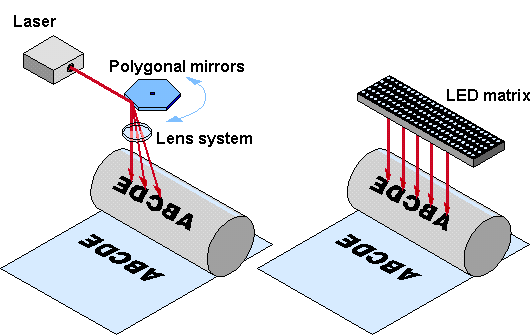
\includegraphics[width=1\linewidth]{TVY-POS/Laserove-a-LED-tiskarny/LEDandLaserPrinter.png}

\section{Rozdělení sítí podle rozsahu}
\section{Výstupní zobrazovací zařízení}
\label{sec:vystupni-zobrazovaci-zarizeni}
Úkolem těchto zařízení je předat informaci uživateli pomocí grafického prostředí.
Do PC je možné tyto zařízení připojit digitálně (HDMI, DisplayPort) či analogově (VGA).
Mezi základní parametry těchto zařízení patří:\\ \\
\begin{tabularx}{\linewidth}{l|l|l}
  \textbf{Parametr}    & \textbf{Jednotka} & \textbf{Popis}                                               \\
  \hline
  Úhlopříčka           & '' (Palce)        & Velikost vzdálenosti mezi protilehlými rohy obrazovky        \\
  \hline
  Rozlišení            & Pixel na pixel    & Počet možných zobrazitelných bodů na výšku a na šířku        \\
  \hline
  Obnovovací frekvence & Hz                & Udává kolikrát za sekundu je obrazovka překreslována         \\
  \hline
  Doba odezvy          & ms                & Udává dobu za kterou se snímek zaslaný na obrazovku vykreslí \\
  \hline
  Spotřeba energie     & W                 & Udává spotřebu energie (Plasma, Crt >> LCD)                  \\
  \hline
  Možnost připojení    & ---               & VGA, DVI, HDMI, DisplayPort, USB-C                           \\
\end{tabularx}
\subsection{Technologie}
Různé technologie využívají jiný způsob zobrazení výsledného obrazu.
Liší se mezi sebou spotřebou, barvama a životností.
\subsubsection{CRT}
Obrazovka monitoru je tvořena velkou elektronkou.
Na jedné straně anoda (obrazovka) a na druhé žhavená katoda (Elektronové dělo).
Vnitřní strana obrazovky je luminofor, který po dopadu elektronu vytvoří světlo.
Pro rosvícení elektronů na správném místě se používá mřížka.
Obraz je vykreslován po řádcích horizntálně vychylován pomocí elektromagnetu.
Obsahuje tři samostatná děla pro každou z barev RGB.
Má vysoký kontrast a dokonalou černou.
Celý monitor je velmi těžký, má vysokou spotřebu a kvůli vypouklé obrazovce zkresluje obraz.
\subsubsection{Plasma}
Jedná se o dvě skleněné desky mezi nimiž leží komůrky s elektrodou se směší plýnů neonu a xenonu.
Po zapnutí elektroda přivede do plynu proud a v plazmě se uvolní volné eketrony.
Poté co se ionty začnou tímto způsobem srážet, tak začnou uvolňovat fotony.
Světlo si takto displej vytváří sám a nepotřebuje k tomu samostatný zdroj.
Na čelní straně každé takové komůrky pak začnou zářit červenou, zelenou nebo modrou barvou.
Na každý pixel jsou takto tři elektrony každý pro jednou barvu.
\subsubsection{LCD}
Technologie tekutých krystalů.
Chemická látka pod vlivem elektrického pole mění svojí molekulární strukturu podle které určují množství procházející světla.
Chová se jako kapamtila ale optické vlastnosti má krystalických látek, je složena z podlouhlých molekul orientovaných v jednom směru.
Každý pixel se skládá z molekul takových tekutých krystalů mezi dvěma elektrodami a polarizačními filtry.
Osy filtrů jsou na sebe kolmé.
Bez krystalů by světlo prošlo jedním filtrem, ale bylo by blokováno druhým.
Světlo je generováno pomocí buďto pasivního (Venkovní světlo) nebo aktivního zdroje světla za krystaly (LED).
Každý pixel je rozdělen na tři subpixely pro RGB.
Používají se dvě technolgie:\\
\begin{description}
  \item[TN]- Světlo bez natočení krystalů projde. Starší technologie.
  \item[IPS]- Světlo bez natočen krystalů neprojde. Novější technologie. Lepší barvy a pozorovací úhly.
\end{description}
\subsubsection{OLED}
Technologie organických (založené na uhlíku) elektroluminiscenčních diod.
Po zavedení proudu diody vyzařují světlo.
Možnost využití pro tenký a pružný displej, ejlikož mezi anodou a katodou je luminofor, který po průchodu elektronů vyzařuje fotony.
Má široké pozorovací úhly, vysoký jas, rychlou odezvu, dobrý konstrast a skutečnou černou barvu.
Má menší životnost oproti LCD a může dojít k vypálení obrazovky.
\subsubsection{Projektory}
Zařízení které zobrazuje obraz na ploše nikoly na displayi.
Využívá pro velké místnosti, jelikož jsme takto jednoduše schopni zobrazit obraz i na metrové plochy.
Existují dva druhy projektorů.
Buďto bílé světlo z lampy dopadá pomocí rotujícího kotouše na soustavu poloprostustných zdrcadel nebo projektor obsahuje tři LCD displeje, každý pro barvu jednu RGB, který potom pomocí optické soustavy promítá.
LCD má větší ostrost obrazu.\\
\begin{multicols}{2}
  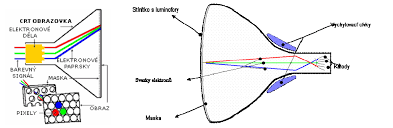
\includegraphics[width=\linewidth]{TVY-POS/Vystupni-zobrazovaci-zarizeni/crt.png}
  \columnbreak
  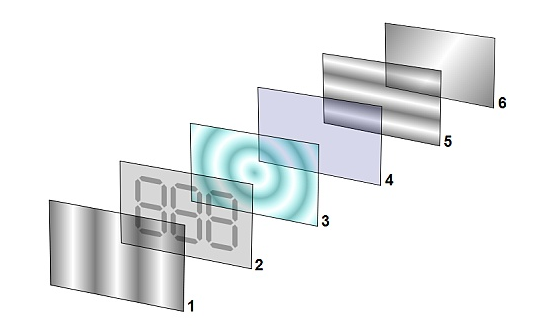
\includegraphics[width=\linewidth]{TVY-POS/Vystupni-zobrazovaci-zarizeni/lcd.png}
\end{multicols}
\begin{multicols}{2}
  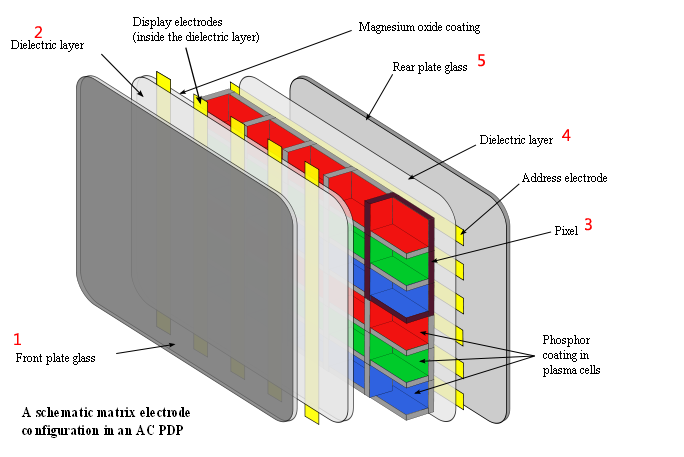
\includegraphics[width=\linewidth]{TVY-POS/Vystupni-zobrazovaci-zarizeni/plasma.png}
  \columnbreak
  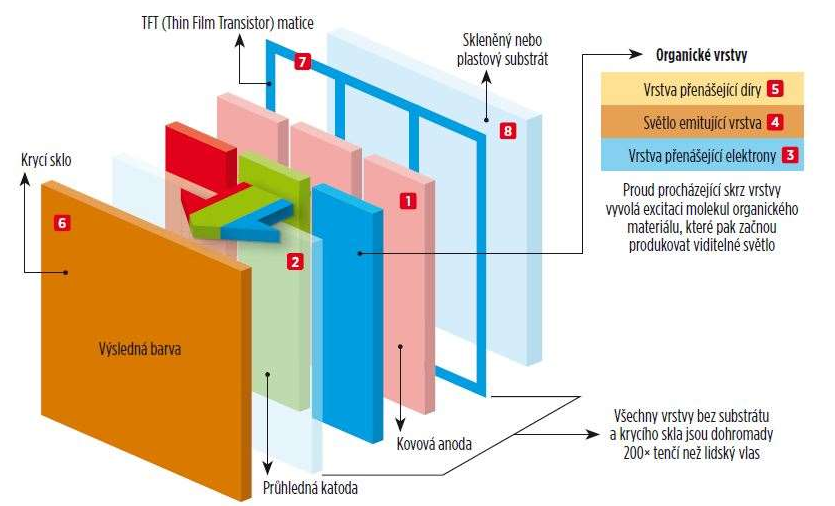
\includegraphics[width=\linewidth]{TVY-POS/Vystupni-zobrazovaci-zarizeni/oled.png}
\end{multicols}
\begin{center}
  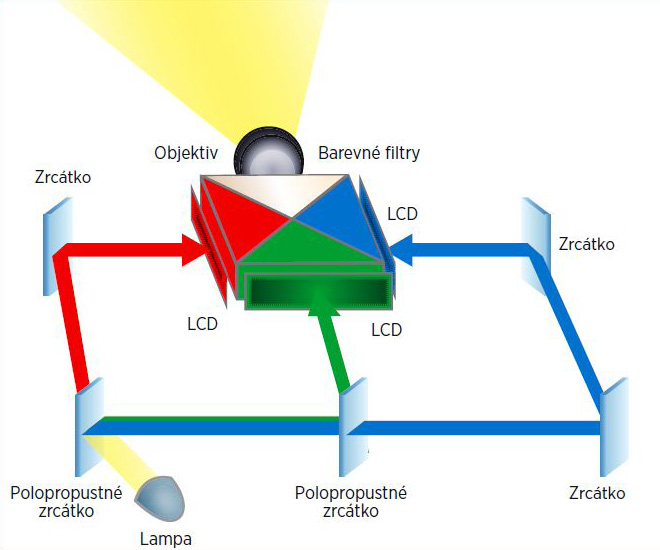
\includegraphics[width=0.5\linewidth]{TVY-POS/Vystupni-zobrazovaci-zarizeni/lcd-projektor.jpg}
\end{center}

\section{Hrozby na síti}
\label{sec:hrozby-na-siti}
Hrozby můžou být software či hardware sestrojené za účelem odcizení dat, peněz, informací nebo k zablokování přístupu.
Je nutné se proti tumto bránit na všech vrstvách ISO/OSI.
Mezi takové hrozby může patřit:
\begin{itemize}
  \item SW
        \begin{itemize}
          \item Viry - bez vědomí uživatele spouští v PC operace
          \item Malware - zajišťuje tajný přístup do zařízení
        \end{itemize}
  \item HW
        \begin{itemize}
          \item Sniffer - zařízení pro sběr dat
          \item Backdoor - brána pro připojení do sítě
        \end{itemize}
\end{itemize}
\subsection{Dělení malware}
\begin{description}
  \item[Spyware]- Odesílá uživatelovi data bez jeho vědomí.
  \item[Adware]- Odstranění agresivní reklamy za poplatek.
  \item[Phishing]- Stránka vydávající se za jinou. Po zadání přihlašovacích údajů se odešlou hackerovi.
  \item[Trojský kůň]- Funkční program, který obsahuje skrytý vir.
  \item[Červ]- Samo šířící se malware. Má v sobě zabudovanou šířící se funkci.
  \item[Keylogger]- Každý stisk klávesy se zaznamenává a odesílá zkrze internet hackerovi.
  \item[Ransomware]- Zašifruje disk a pro dešifraci je nutné zaplatit poplatek.
\end{description}
\subsection{Šíření malware}
\begin{itemize}
  \item Mailem - jako příloha, například pod falešnou identitou úřadu, policie\dots
  \item Trojský kůň
  \item Červ
\end{itemize}
\subsection{Odstranění malware}
\begin{enumerate}
  \item Odinstalace programu
  \item Odstavit vir pomocí antiviru
  \item Reinstalace OS
\end{enumerate}
\subsection{Druhy útoků}
\begin{description}
  \item[Brute force]- Snaha o prolomění ochrany hrubou silou. Zkoušení všech možných kobinací hesel. 
  \item[Social engineering]- Snaha o získání přístupu pomocí samotné interakce s uživatelem.
  \item[DNS spoofing]- DNS špatně přeloží adresu na adresu hackera, který poté získá údaje. (Phishing)
  \item[DDOS]- Vyřazení služby z provozu. Zahlcení infrastruktury provozem co není schopen zvládnout.
  \item[BOTnet]- Pomocí jednotlivě nakažených PC hacker provádí útoky ve vetším množství.
\end{description}
\section{Aritmetické operace v počítači}
\section{FW a ochrany jednotlivých vrstev TCP/IP}
\section{Vstupní zařízení}
\subsection{Klávesnice}
Klávesenice předává informace o stlačených klávesách operačnímu systému zpracované BIOSem.
Připojují se fyzicky pomocí USB a PS2 konektoru nebo bezdrátově pomocí Bluetooth či infračerveného záření.
Informace jsou ve SCAN kódu, kde se začíná klávesou ESC na čísle 1 a pokračuje se dál po řádcích.
Postup přenosu stisku:
\begin{enumerate}
  \item Mikroprocesor vestavěný do klávesnice nebo základové desky neustále monitoruje stav klávesnice
  \item Změna stavu způsobí vysílání kódu do základové desky klávesnice
  \item Stisk musí trvat aspoň 2 nebo 3 cykly, jinak se ignoruje
  \item Po uvolnění klávesy se kód klávesy zvýší o 128
  \item Číslo se uloží do paměti klávesnice a mikroprocesorem se zapíše na port
  \item Nastane přerušení a BIOS čte kód klávesy
  \item Po přečtení BIOS sdělí klávesnici pokyn o vymazání klávesy
  \item Při delším stisku se generuje signál stlačené klávesy
  \item BIOS dále testuje ještě 2 byty klávesnice na portu pro případné speciální funkce jako CTRL, ALT, aj.\\
        Tyto funkce se zapisují do bytů na adrese 0417H a 0418H
\end{enumerate}
\subsubsection{Mechanické klávesnice}
Potlačením tlačítka se mechanicky spojí vodiče. Pružinou se klávesa vratí zpátky.\\
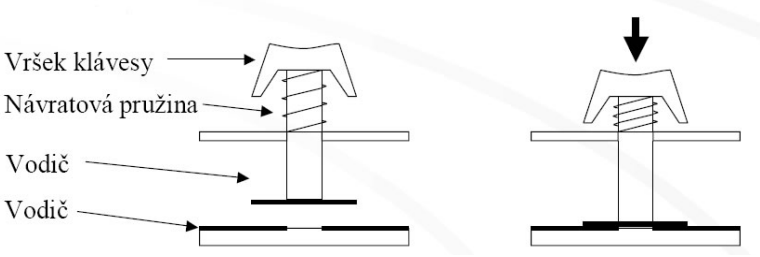
\includegraphics[width=1\linewidth]{TVY-POS/Vstupni-zarizeni/mechanickey.png}
\subsubsection{Membránové klávesnice}
Protlačením membrány dojde ke styku kontaků. Většinou pomocí mikrospínačů.\\
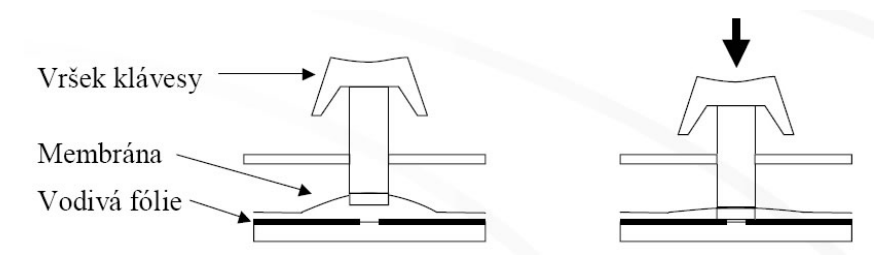
\includegraphics[width=1\linewidth]{TVY-POS/Vstupni-zarizeni/membranekey.png}
\subsubsection{Kapacitní klávesnice}
Přiblížení jádra k dorazu změní kapacitu kondnzátoru.
Není zde žádný dotek.
Jádrem je dielektrikum, které je pružinou oddalování.\\
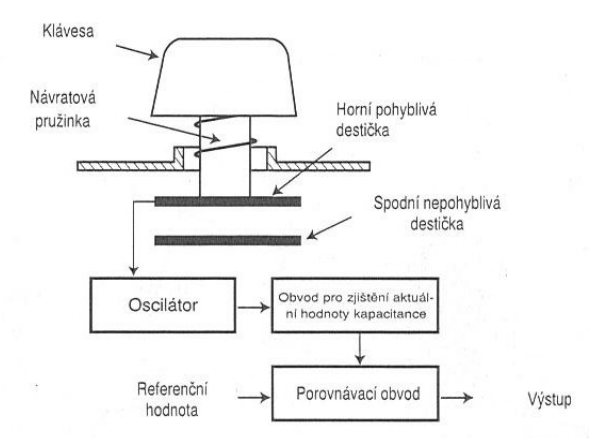
\includegraphics[width=1\linewidth]{TVY-POS/Vstupni-zarizeni/capacitorkey.png}
\subsubsection{Hallovy klávevy}
Klávesy mají uvnitř permanentní magnet.
Pod klávesou je Hallova sonda, která reguje za změnu magentického pole.
Při stisku klávesy se magnet přiblíží k Hallově sondě, která jako reakci vyšle elektrický signál.
Změnou magnetického pole pohybem klávesy se změní napětí na výstupu.
Takové klávesnice jsou velmi kvalitní, ale drahé.
\subsubsection{Dotykové klávesnice}
Dotyky se detekují pomocí změny kapacity kondenzátoru změnou dielektrika, který představuje prst.
Bez pohyblivých částí.
\subsection{Tablety}
Jsou to snímací podložky funkčně podobné grafickým stolům.
Využívají se ke kreslení vektorových obrazců.
Po podložce se pohybuje snímací zařízení, většinou myš se zaměřovačem nebo pero.
Myš místo kuličky obsahuje vysílací cívku, která vysílá impulsy čtené podložkou pomocí sítě snímačů.
Obsahuje lupu pro přenou polohu a tlačítka.
V peru bývá tlakový senzor pro určení tloušťky čáry.
\subsection{Světelná pera (Optická, Light Pen)}
Světelné pero snímá pozici pera na monitoru pomocí grafického adaptéru.
V peru je snímač světla, který identifikuje polohu pomocí bodu na monitoru.
Pracuje s informací, kdy se bod na monitoru obnoví, pomocí které určí, kde se pero nachází.
Monitor musí obraz vysílat řádek po řádku, bod po bodu.
\subsection{Dotykové obrazovky}
Existuje několik druhů dotykových obrazovek
\subsubsection{Rezistivní displeje}
Obrazovku tvoří pružná membrána.
Stiskem membrány spojíme elektrický proud.
Na základě velikosti jednotlivých proudů se vypočítá poloha displeje.
\subsubsection{Kapacitní dotykové dispeje}
Funguje na základě vodivosti lidského těla.
Dotykem prstu na displej se uzavře elektrický obvod a vytvoří se kapacita.
Řadič na základě velikosti kapacity určí polohu prstu.
\subsubsection{Dotykové displeje s IR}
Kolem displeje je rám vysílající IR paprsky.
Vsunutím předmětu se paprsek na daném místě přeruší.
\subsubsection{Displej s povrchovou akustickou vlnou (SAW)}
V rozích displeje jsou vysílače a přjímače 5Mhz sígnálu.
Přijímače vyhodnucují změnu šíření těchto vln a podle toho vyhodnutí polohu rušení.
Problematická je citlivost, jelikož malé znečištění je stále fatální.
\subsection{Myši}
Je to malé polohovací zařízení, která přenáší informace o svém pohybu do počítače.
Většinou se toto projeví jako pohyb kruzoru.
Mívá tlačíka a kolečko.
Připojovala se pomocí sériového RS-232 portu, poté se používal PS/2 a nyní USB.
Některé myši se dají pomocí redukce připojit do PS/2 či USB.
Existují i bezdrátové myši, u kterých se využívá buďto IR (IrDA) nebo rádiových vln (Např.: Bluetooth).
\subsubsection{Mechanická myš (Kuličková)}
Zespod myši je kulička, která se pohybem roztáčí.
Otáčení kuličky snímají dvě navzájem kolmé hřídele.
Hřídele při svém pohybu přenáší pohyb na otočnou clonu ve tvaru kruhu s okny.
Každé pootočení clony přeruší paprsek, což je přeneseno na elektrický impulz.
Rozpoznává se směr otáčení pomocí Grayova kódu.
Impulzy myši tvoří 2 a 2 bity, která se pak převádí na pohyb po X a Y na obrazovce.
\subsubsection{Optická myš}
Myš vysílá LED nebo laser, který se snímá fotodiodami nebo jiným optickým snímačem.
Pohyb myši se poté v reálném čase převádí do os X a Y.
Infračervené záření má vyšší přesnost a nižší spotřebu, ale ve skutečnosti na světle nezáleží.
Myš funguje lépe na strukturovaném povrchu, kde je možné snadno rozpoznat pohyb podkladu.
\end{document}
